\chapter{Quantification of incomparability for sets of states} \label{chap:volume}

This chapter is a direct continuation of Chapter \ref{chap:incomparability}. The question that this chapter tries to answer is the following: how can we generalize the notion of incomparability function of a probe state, relative to a \textit{set of reference states} ? For the rest of this master thesis, we will call this set of reference states the \textit{bank}. Because we are interested in quantum applications and LOCC transformations, which are confined to the $\mathcal{T}_+$ sets, we will only discuss the generalization of $E^+$. We did not attempt it, but we believe that reversing the whole discussion of this chapter is also possible for other theories such as quantum thermodynamics, which work with the $\mathcal{T}_-$ sets instead.% We suspect that this might require to use a negentropy-based $E^-$.



\section{Entropic volume of majorization cones}

\subsection{Venn diagrams and the inclusion-exclusion principle}

Let us remain in the 2 state context for now. Incomparability seems to enable \textit{diversity} in the set of LOCC-reachable states from $p$ and $q$. In some sense, we would expect $E^+$ to characterize how many states are only accessible from $p$, but not from $q$. The set-theoretic intuition is helpful here: we are looking to compute the volume (which is directly linked to the amount of reachable states) $V(\mathcal{T}_+(p) \backslash \mathcal{T}_+(q))$, where $V$ is a measure that sends the cone of a state to a real number. For sets $A$ and $B$, set theory gives us the following expression

\begin{equation} \label{eq:2_set_exclusion}
    V(A \backslash B) = V(A) - V(A \cap B),
\end{equation}

\noindent which is illustrated with Venn diagrams in Figure \ref{fig:venn_two}.

\begin{figure}[h!] % code adapted from https://texample.net/venn-diagram/
    \centering
    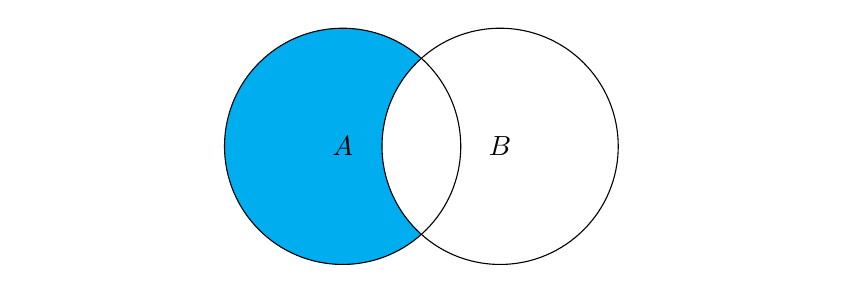
\begin{tikzpicture}
        \begin{scope}[even odd rule]
            \clip (0:1cm) circle (1.5cm) (-5, -1.5) rectangle (5, 1.5);
            \fill[cyan] (180:1cm) circle (1.5cm);
        \end{scope}
        \draw (180:1cm) circle (1.5cm) node [text=black] {$A$};
        \draw (0:1cm) circle (1.5cm) node [text=black] {$B$};
        %\draw \thirdcircle node [text=black,below right] {$C$};
    \end{tikzpicture}
    \caption{Venn diagram of two sets $A, B$ with non-empty intersection. $A \backslash B$ is colored in cyan.}
    \label{fig:venn_two}
\end{figure}

The key insight which we will use extensively for this chapter, which to our knowledge has not been used in the QRT field before, is that $\mathcal{T}_+(p) \cap \mathcal{T}_+(q) = \mathcal{T}_+(p \vee q)$ (we had briefly mentioned this relationship in Figure \ref{fig:meet_join_example}). It is very important to note at this stage that while visually similar, the notation for the lattice-theoretic meet and join $\wedge$ and $\vee$ should not be confused with the notations for the set-theoretic union and intersection $\cup$ and $\cap$. With this insight, we can rewrite Eq. (\ref{eq:2_set_exclusion}) with $A = \mathcal{T}_+(p)$ and $B = \mathcal{T}_+(q)$ as

\begin{equation}
    V(\mathcal{T}_+(p) \backslash \mathcal{T}_+(q)) = V(\mathcal{T}_+(p)) - V(\mathcal{T}_+(p \vee q)).
\end{equation}

Thankfully, it is possible to generalize this idea further. For example, for three sets $A, B, C$ we have the statement

\begin{equation}
    V(A \backslash (B \cup C)) = V(A) - V(A \cap B) - V(A \cap C) + V(A \cap B \cap C),
\end{equation}

\noindent which is illustrated with Venn diagrams in Figure \ref{fig:venn_three}.

\begin{figure}[h!] % code adapted from https://tex.stackexchange.com/questions/9681/how-to-draw-venn-diagrams-especially-complements-in-latex
    \centering
    \begin{tikzpicture}
        \begin{scope}
            \fill[cyan] \firstcircle;
        \end{scope}
        \begin{scope}
            \clip \firstcircle;
            \fill[white] \secondcircle;
        \end{scope}
        \begin{scope}
            \clip \firstcircle;
            \fill[white] \thirdcircle;
        \end{scope}
        \draw \firstcircle node[text=black,above] {$A$};
        \draw \secondcircle node [text=black,below left] {$B$};
        \draw \thirdcircle node [text=black,below right] {$C$};
    \end{tikzpicture}
    \caption{Venn diagram of three sets $A, B, C$ with non-empty intersections. $A \backslash (B \cup C)$ is colored in cyan.}
    \label{fig:venn_three}
\end{figure}

The idea is essentially that when removing both $A \cap B$ and $A \cap C$ from $A$, the region $A \cap B \cap C$ gets removed twice, and we must add it back to get the correct set size. This formula can then be rewritten with $A = \mathcal{T}_+(p)$, $B = \mathcal{T}_+(q_1)$ and $C = \mathcal{T}_+(q_2)$ to compute the volume of the region that is \textit{only} LOCC-reachable from $p$, and not from the bank $\{q_1, q_2\}$. The fully general set-theoretic formula is known as the \textit{inclusion-exclusion principle}, which gives the following statement.

\begin{theorem}[{Inclusion-exclusion principle \cite[p. 99]{tao_introduction_2011}}] \label{th:inclusion-exclusion}
    Let $A_i \subseteq \Omega, 0 \leq i \leq k$, and let $V$ be a measure over $\Omega$. We have
    \begin{equation}
        V\left(A_0 \backslash \left(\bigcup\limits_{i = 1}^k A_i\right)\right) = V(A_0) + \sum_{\emptyset \neq J \subseteq \{1, \dots, k\}} (-1)^{|J|} \: V\left(A_0 \bigcap\limits_{i \in J} A_i\right),
    \end{equation}
    where the sum $\sum_{\emptyset \neq J \subseteq \{1, \dots, k\}}$ denotes the sum over all possible combinations $J$ of elements from $\{1, \dots, k\}$ (excluding the combination with no elements) and where $|J|$ denotes the cardinality of the set $J$.
\end{theorem}

Several equivalent versions of Theorem \ref{th:inclusion-exclusion} exist, but this version is the relevant one in our context. We propose the following corollary.

\begin{corollary}[LOCC inclusion-exclusion] \label{corr:LOCC_inclusion-exclusion}
    Let $p, q_1, \dots, q_k \in \mathcal{P}^d$, and let $V$ be a measure over $\mathcal{P}^d$. Then
    \begin{equation} \label{eq:LOCC_inclusion-exclusion}
        V\left(\mathcal{T}_+(p) \backslash \left(\bigcup\limits_{i = 1}^k \mathcal{T}_+(q_i)\right)\right) = V\left(\mathcal{T}_+(p)\right) + \sum_{\emptyset \neq J \subseteq \{1, \dots, k\}} (-1)^{|J|} \: V\left(\mathcal{T}_+\left(p \bigvee\limits_{i \in J} q_i\right)\right),
    \end{equation}
    where $p \bigvee\limits_{i \in J} q_i$ is defined as $p \vee q_{j_1} \vee \dots \vee q_{j_n}$ (with $\{j_1, \dots, j_n\} = J$), is the volume of the set of states that is only LOCC-reachable from $p$ but not from the bank of states $\{q_1, \dots, q_k\}$.
\end{corollary}



\subsection{Generalization of incomparability monotones to a bank of states}

The volume of convex polytopes in Weyl chambers (which our majorization cones are) under a Euclidean measure can be computed explicitly. Unfortunately, no closed-form solution exists past dimension 3, although algorithms do exist to compute them in any dimension \cite{junior_geometric_2022}. However, compute time and memory requirements can quickly become limiting as the dimensions increase, rendering exact methods difficult to use \cite{bueler_exact_2000}.

There is an additional difficulty in the field of LOCC transformations: quantum states are not distributed evenly on the canonical Weyl chamber of a $\Delta_{d-1}$ simplex. This is because the Schmidt decomposition induces a non-euclidean measure, called a Haar measure (which essentially captures the density of quantum states in the Schmidt vector space). Volume formulae taking this Haar measure into account do exist, and are useful in quantifying things like the average entanglement in a region of density matrices \cite{zyczkowski_induced_2001}.

However, we will not study them further in this master thesis. Indeed, in terms of an entanglement QRT, it is not entirely clear why a Schmidt vector shared by many quantum states should be weighted more than a Schmidt vector that is shared by few quantum states. This is because states with the same Schmidt vector are equivalent up to a local change of basis, and can thus be interchanged without losing any resource. Of course, we are not trying to argue that assigning a non-uniform weight to Schmidt vectors is necessarily useless, but rather that it is not clear why there couldn't exist other relevant choices of weighting than the density of LOCC-equivalent quantum states.

With this in mind, we postulate that the Shannon entropy is itself a measure of the volume of majorization cones under some unknown measure. This makes our future incomparability monotone $E^+(p \parallel q) = H(p) - H(p \vee q)$ from Chapter \ref{chap:incomparability} much easier to interpret: according to Eq. (\ref{eq:unique_entropy}) it measures the volume of states that are reachable from $p$, but not from $q$. For this reason, it is perhaps more natural to call $E^+$ the \textit{uniqueness entropy}. We propose the following generalization of $E^+$.

\begin{definition}[Uniqueness entropy] \label{def:unique_entropy}
    Let $p, q_1, \dots, q_k \in \mathcal{P}^d$. The uniqueness entropy of $p$ relative to the bank $\{q_1, \dots, q_k\}$, which we note $E^+(p \parallel q_1, \dots, q_k)$, is defined as 
    \begin{equation} \label{eq:unique_entropy}
        E^+(p \parallel q_1, \dots, q_k) = H(p) + \sum_{\emptyset \neq J \subseteq \{1, \dots, k\}} (-1)^{|J|} \: H\left(p \bigvee\limits_{i \in J} q_i\right).
    \end{equation}
\end{definition}

A simple example with three states gives $E^+(p \parallel q_1, q_2) = H(p) - H(p \vee q_1) - H(p \vee q_2) + H(p \vee q_1 \vee q_2)$. This is better understood with the cone diagram in Figure \ref{fig:3_cone_example} (which now has a new Venn-like interpretation).

\begin{figure}[h!]
    \centering
    \begin{tikzpicture}[scale=0.9]
        % draw cone of q1
        \coordinate (Q1) at (1.5, 3.75);
        \coordinate (Q1L) at (-1, 0);
        \coordinate (Q1R) at (4, 0);
        \draw [name path=Q1--Q1L] (Q1) -- (Q1L);
        \draw [name path=Q1--Q1R] (Q1) -- (Q1R);
        \node [fill=black,inner sep=1pt,label=90:$q_1$] at (Q1) {};
        % draw cone of q2
        \coordinate (P) at (4, 4.5);
        \coordinate (PL) at (1, 0);
        \coordinate (PR) at (7, 0);
        \draw [name path=P--PL] (P) -- (PL);
        \draw [name path=P--PR] (P) -- (PR);
        \node [fill=black,inner sep=1pt,label=90:$p$] at (P) {};
        % draw cone of q3
        \coordinate (Q2) at (5.5, 4.5);
        \coordinate (Q2L) at (2.5, 0);
        \coordinate (Q2R) at (7, 2.25);
        \draw [name path=Q2--Q2L] (Q2) -- (Q2L);
        \draw [name path=Q2--Q2R] (Q2) -- (Q2R);
        \node [fill=black,inner sep=1pt,label=90:$q_2$] at (Q2) {};
        % intersections
        \path [name intersections={of=P--PL and Q1--Q1R,by=PVQ1}];
        \path [name intersections={of=P--PR and Q2--Q2L,by=PVQ2}];
        \path [name intersections={of=Q1--Q1R and Q2--Q2L,by=PVQ1VQ2}];
        \node [fill=black,inner sep=1pt] at (PVQ1) {};
        \node [inner sep=1pt, label=180:$p \vee q_1$] at (PVQ1) {};

        \node [fill=black,inner sep=1pt,label=0:$p \vee q_2$] at (PVQ2) {};
        \node [fill=black,inner sep=1pt,label=0:$p \vee q_1 \vee q_2$] at (PVQ1VQ2) {};

        \fill[fill=red, opacity=0.2] (P) -- (PVQ1) -- (PVQ1VQ2) -- (PVQ2) -- cycle;
        %\node [inner sep=0pt, label=270:{$E^+(p \parallel q_1, q_2)$}] at ($ (P) !.25! (PVQ1) !.25! (PVQ1VQ2) !.25! (PVQ2) $) {};


    \end{tikzpicture}
    \caption{Geometric representation of the uniqueness entropy $E^+(p \parallel q_1, q_2)$ (shaded in red) for 3 states $p, q_1, q_2 \in \mathcal{P}^d$. The analogy with Figure \ref{fig:venn_three} is quite clear: we add back $H(p \vee q_1 \vee q_2)$ because it is already removed twice in the formula.}
    \label{fig:3_cone_example}
\end{figure}

A small overview of the essentials of measure theory is available in Appendix \ref{app:measure_theory}. We will also denote the set of all future majorization cones by $\mathbb{T}_+$. While this definition and postulate may not seem too far-fetched considering the previous discussion, this essentially means that if $E^+$ behaves like a volume, then a set function $\mu_0$ which sends cones onto the entropy of their tip $p$ is a valid measure of the set $\mathcal{P}^d$. In other words, the volume of a cone would be entirely determined by its tip (meaning that $\mu_0$ would be an unusual set function). That this might be possible is not too surprising however, because existing formulae for computing the volume of convex polytopes already only use the vertices of the polytope \cite{braden_surveyors_1986}. Moreover, algorithms to compute the location of the vertices of the majorization cone of any vector $p$ do exist, and Ref. \cite{junior_geometric_2022} even provides a Mathematica implementation\footnote{\url{https://github.com/AdeOliveiraJunior/Thermal-Cones}} (in the context of thermomajorization\footnote{It is interesting to note at this point that the volume of thermal cones has already been studied in Ref. \cite{junior_geometric_2022}, and that they also give an interpretation of the volume being akin to a resource. Moreover, they also propose a euclidean and Haar volume for entanglement cones. However, they studied the volume of individual cones, and thus did not attempt to characterize the volume uniquely accessible from a state.} which is similar). Therefore, the volume of a majorization cone is entirely determined by its tip.

Some work did go into studying the basics of measure theory and defining a rigorous set function which would send cones onto the entropy of their tip, which would then be a valid measure for majorization cones if it could verify the properties of countable additivity and positivity on the $\sigma$-algebra (cf. Def. \ref{def:sigma_algebra}) generated by the majorization cones. Such a result would be very interesting, and would give new insight into the nature of entropy on the majorization lattice.

For this to be possible we need our set function to work on a given collection of subsets of $\mathcal{P}^d$ of interest. We are only really interested in the measure of the cones, however a rigorous measure must at least be defined on a $\sigma$-algebra. We can generate the $\sigma$-algebra from the true collection of interest: the $\sigma$-algebra of our majorization cones contains all the possible unions, complements and intersections of cones. Intersections are easy because $\mathcal{T}_+(p) \cap \mathcal{T}_+(q) = \mathcal{T}_+(p \vee q)$ (and so they form a $\pi$-system), but unions and complements of cones are not necessarily cones and so the naive set function which sends cones on the entropy of their tip is not directly defined for those. Moreover, for $\mu_0$ to be a measure, it needs to be countably additive. However, countable additivity can only be shown for disjoint sets, but the set of future cones does not contain a single pairwise disjoint set\footnote{No future cone is disjoint because they are all guaranteed to at least contain $\overline{\delta}_d \coloneqq (1, 0, \dots, 0)$.} (but the $\sigma$-algebra generated from the majorization cones $\sigma(\mathbb{T_+})$ does contain disjoint sets). It is unfortunately not clear if and how one could extend the naive set function to $\sigma(\mathbb{T_+})$. We believe that a recursive definition for an extended set function $\mu_{\text{ext}}$ sending a set $A$ to $\mu_0(A)$ if $A$ is a cone, and to $\mu_{\text{ext}}(A') +\mu_{\text{ext}}(A'') - \mu_{\text{ext}}(A' \cap A'')$ if $A$ is the union of 2 sets $A'$ and $A''$ might be enough, however proving countable additivity for such a recursive function seemed out of scope for this master thesis and was not studied further.



\subsection{Expected properties} \label{sec:unique_entropy_properties}

Unfortunately, without a clear set function we cannot work on showing finite additivity, and so we will not show that an entropy-based set function is rigorously a volume. However, we will still attempt to show that our uniqueness entropy $E^+$ holds properties compatible with the geometrical intuition one could have for such a volume. For any $p, q_1, \dots, q_k, q_{k+1} \in \mathcal{P}^d$, we have

\begin{enumerate}
    \item \textbf{Commutativity:} $E^+(p \parallel q_1, \dots, q_i, \dots, q_j, \dots, q_k) = E^+(p \parallel q_1, \dots, q_j, \dots, q_i, \dots, q_k)$ for any $i \neq j$. \label{prop:commutativity}
    \item \textbf{Empty volume:} $E^+(\overline{\delta}_d \parallel q_1, \dots, q_k) = 0$. \label{prop:empty}
    \item \textbf{Absorption in $p$:} $E^+(p \parallel q_1, \dots, q_k) = 0$ if $\exists i \leq k \: | \: p \succ q_i$. \label{prop:p_absorption}
    \item \textbf{Absorption in $q$:} $E^+(p \parallel q_1, \dots, q_k, q_{k+1}) = E^+(p \parallel q_1, \dots, q_k)$ if $\exists i \leq k \: | \: q_{k+1} \succ q_i$. \label{prop:q_absorption}
    \item \textbf{Positivity:} $E^+(p \parallel q_1, \dots, q_k) \geq 0$. \label{prop:positivity}
    \item \textbf{Increasing monotonicity in $p$:} $E^+(Dp \parallel q_1, \dots, q_k) \geq E^+(p \parallel q_1, \dots, q_k)$ for any bistochastic matrix $D$. \label{prop:p_monotonicity}
    \item \textbf{Decreasing monotonicity in $q$:} $E^+(p \parallel q_1, \dots, Dq_i, \dots, q_k) \leq E^+(p \parallel q_1, \dots, q_i, \dots, q_k) \: \forall i \leq k$,  for any bistochastic matrix $D$. \label{prop:q_monotonicity}
\end{enumerate}

\noindent The key insight needed to prove these properties is given by the following lemma (proven in Appendix \ref{app:unique_entropy_properties}), which lends itself very well to induction proofs.

\begin{lemma} \label{lem:induction_trick}
    Let $p, q_1, \dots, q_k, q_{k+1} \in \mathcal{P}^d$. Then,
    \begin{equation}
        E^+(p \parallel q_1, \dots, q_k, q_{k+1}) = E^+(p \parallel q_1, \dots, q_k) - E^+(p \vee q_{k+1} \parallel q_1, \dots, q_k).
    \end{equation}
\end{lemma}

It turns out that only Props. \ref{prop:positivity}, \ref{prop:p_monotonicity} and \ref{prop:q_monotonicity} are difficult to prove. The other proofs come fairly naturally from Definition \ref{def:unique_entropy}, see Appendix \ref{app:unique_entropy_properties}. Note that Prop. \ref{prop:commutativity} implies that the ordering of the bank is arbitrary, and so we can always make any vector the last vector of the bank, which is useful for proving Props. \ref{prop:p_absorption}, \ref{prop:q_absorption} and \ref{prop:q_monotonicity} as showing the property for $i = k$ is sufficient. In order to prove Props. \ref{prop:positivity}, \ref{prop:p_monotonicity} and \ref{prop:q_monotonicity}, we will need an additional small lemma.

\begin{lemma} \label{lem:idempotency_trick}
    Let $p, q_1, \dots, q_k, \in \mathcal{P}^d$. Then,
    \begin{equation}
        E^+(p \parallel q_1, \dots, q_{k-1}, q_k) = E^+(p \parallel q_1, \dots, q_{k-1}, p \vee q_k).
    \end{equation}
\end{lemma}
\begin{proof}
    Immediate from commutativity, associativity and idempotency of the join (cf. Section \ref{sec:algebraic_properties}).
\end{proof}

\begin{theorem}[Monotonicity in $p$ and $q$ of the uniqueness entropy] \label{th:double_monotonicity_uniqueness}
    Let $p, q_1, \dots, q_k \in \mathcal{P}^d$. Then, for any bistochastic matrix $D$, $E^+$ is an increasing monotone in $p$ and a decreasing monotone in $q$. Formally,
    \begin{equation}
        \begin{system}
            E^+(p \parallel q_1, \dots, q_k) \leq E^+(Dp \parallel q_1, \dots, q_k)\\
            E^+(p \parallel q_1, \dots, q_k) \geq E^+(p \parallel q_1, \dots, Dq_k).
        \end{system}
    \end{equation}
\end{theorem}

\begin{proof}
    We will do an induction proof. Let us first assume that $E^+(p \parallel q_1, \dots, q_i)$ is monotonically decreasing in $q$ for some value of $i$, and let us show that this property then propagates to $i+1$, meaning that $E^+(p \parallel q_1, \dots, q_i, q_{i+1}) - E^+(p \parallel q_1, \dots, q_i, Dq_{i+1}) \geq 0$. First, by using Lemma \ref{lem:induction_trick}, for any bistochastic matrix $D$ we get
    \begin{align}
        &E^+(p \parallel q_1, \dots, q_i, q_{i+1}) - E^+(p \parallel q_1, \dots, q_i, Dq_{i+1})\nonumber \\
        = \: &E^+(p \parallel q_1, \dots, q_i) - E^+(p \vee q_{i+1} \parallel q_1, \dots, q_i) - E^+(p \parallel q_1, \dots, q_i)\nonumber\\
        &\: +  E^+(p \vee Dq_{i+1} \parallel q_1, \dots, q_i)\\
        = \: &E^+(p \vee Dq_{i+1} \parallel q_1, \dots, q_i) - E^+(p \vee q_{i+1} \parallel q_1, \dots, q_i),
    \end{align}
    which is greater or equal to 0 if $E^+(p \parallel q_1, \dots, q_i)$ is monotonically increasing in $p$ for $i$ (because $p \vee q_{i+1} \succ p \vee Dq_{i+1}$ is true for any $D$ \cite[p. 35]{davey_introduction_2002}). Let us now show that $E^+(p \parallel q_1, \dots, q_i)$ being monotonically decreasing in $q$ for $i$ implies that it is also monotonically increasing in $p$ for $i$. Let us first assume that $p \prec q_i$, i.e. $\exists D' \: | \: D' q_i = p$, and consider the following statement, which is true $\forall \: D$ because of Prop. \ref{prop:q_absorption}.
    \begin{align}
        E^+(Dp \parallel q_1, \dots, q_i, p) &= E^+(Dp \parallel q_1, \dots, D'q_i, p) \\
        \implies E^+(Dp \parallel q_1, \dots, q_i) - E^+(Dp \vee p \parallel q_1, \dots, q_i) &= E^+(Dp \parallel q_1, \dots, q_{i-1}, p)\nonumber\\
        &\quad - E^+(\underbrace{Dp \vee D'q_i}_{=p} \parallel q_1, \dots, q_{i-1}, p)\\
        \implies E^+(Dp \parallel q_1, \dots, q_i) - E^+(p \parallel q_1, \dots, q_i) &= E^+(Dp \parallel q_1, \dots, q_{i-1}, p), \label{eq:monotone_p}
    \end{align}
    where the term $E^+(p \parallel q_1, \dots, q_{i-1}, p)$ vanishes by Prop. \ref{prop:p_absorption}. To show increasing monotonicity in $p$, we only need to show that the RHS of (\ref{eq:monotone_p}) is greater or equal to 0. By hypothesis, we know that $E^+(Dp \parallel q_1, \dots, q_{i-1}, p)$ is monotonically decreasing in $q$. In particular, applied on the vector $p$ in the bank,
    \begin{equation}
        E^+(Dp \parallel q_1, \dots, q_{i-1}, p) \geq E^+(Dp \parallel q_1, \dots, q_{i-1}, Dp) = 0
    \end{equation}
    by Prop. \ref{prop:p_absorption}, and so the RHS of (\ref{eq:monotone_p}) is greater or equal to 0. Moreover, Lemma \ref{lem:idempotency_trick} guarantees that if $q_i$ does not majorize $p$, we can simply replace it with $p \vee q_i$, which does majorize $p$. Therefore, we can lift the $p \prec q_i$ restriction. We have thus shown that if $E^+(p \parallel q_1, \dots, q_i)$ is monotone in $q$ for some value of $i$, then it is too in $p$ for $i$, which implies monotonicity in $q$ for $i+1$. Finally, Theorem \ref{th:monotone_future_q} provides the base case for $i = 1$, and so it is monotonically increasing and decreasing in $p$ and $q$ (respectively) for all $i \in \mathbb{N}$. \qedhere
\end{proof}

\noindent With this new result, the last missing property is easy to show.

\begin{theorem}[Positivity of the uniqueness entropy] \label{th:positivity_uniqueness}
    Let $p, q_1, \dots, q_k \in \mathcal{P}^d$. Then,
    \begin{equation}
        E^+(p \parallel q_1, \dots, q_k) \geq 0.
    \end{equation}
\end{theorem}

\begin{proof}
    Using Lemma \ref{lem:induction_trick}, we have
    \begin{equation}
        E^+(p \parallel q_1, \dots, q_i) = E^+(p \parallel q_1, \dots, q_{i-1}) - E^+(\underbrace{p \vee q_{i}}_{\succ p} \parallel q_1, \dots, q_{i-1}),
    \end{equation}
    which is greater or equal to 0 because of the increasing monotonicity in $p$ (cf. Theorem \ref{th:double_monotonicity_uniqueness}) applied on the second term of the LHS, for any value of $i$. \qedhere
\end{proof}

In the quantum picture, corollaries analoguous to those of Theorems \ref{th:monotone_future_p} and \ref{th:monotone_future_q} are also applicable here, e.g. if the volumic intuition is rigorously proven, an entangled state can never reach more unique states (relative to a bank) after any LOCC transformation than before.



\subsection{New intuition for supermodularity from entropic volumes} \label{sec:supermodularity_intuition}

If one could rigorously prove that an entropy-based set function would give a true measure on the $\sigma$-algebra of majorization cones, then one would immediately have a new proof of supermodularity of the Shannon entropy. This is because any measure $\mu$ is monotone (cf. Theorem \ref{th:measure_properties}), in the sense that for any 2 sets $A, B$, if $A \subseteq B$, then $\mu(A) \leq \mu(B)$. Consider now Figure \ref{fig:volumic_supermodularity}.

\begin{figure}[h!]
    \centering
        \begin{tikzpicture}[scale=0.8]
            % draw cone of p
            \coordinate (P) at (-2.5, 2.25);
            \coordinate (PL) at (-4, 0);
            \coordinate (PR) at (-1,0);
            \draw [name path=P--PL] (P) -- (PL);
            \draw [name path=P--PR] (P) -- (PR);
            \node [fill=black,inner sep=1pt,label=180:$p$] at (P) {};
            % draw cone of q
            \coordinate (Q) at (0,3);
            \coordinate (QL) at (-2, 0);
            \coordinate (QR) at (2,0);
            \draw [name path=Q--QL] (Q) -- (QL);
            \draw [name path=Q--QR] (Q) -- (QR);
            \node [fill=black,inner sep=1pt,label=0:$q$] at (Q) {};
            % draw the meet
            \coordinate (PMQ) at (-1, 4.5);
            \draw [name path=PMQ--P] (PMQ) -- (P);
            \draw [name path=PMQ--Q] (PMQ) -- (Q);
            \node [fill=black,inner sep=1pt,label=90:$p \wedge q$] at (PMQ) {};
            % draw the join
            \path [name intersections={of=P--PR and Q--QL,by=PVQ}];
            \fill[fill=red, opacity=0.2] (P) -- (PL) -- (QR) -- (Q) -- (PVQ) -- cycle;
            \node [fill=black,inner sep=1pt,label=0:$p \vee q$] at (PVQ) {};


        \end{tikzpicture}
        \caption{Depiction of the implication of supermodularity by monotonicity of $\mu$. The region $\mathcal{T}_+(p) \cup \mathcal{T}_+(q)$ is shaded in red. Clearly, $\mathcal{T}_+(p) \cup \mathcal{T}_+(q) \subseteq \mathcal{T}_+(p \wedge q)$, with equality iff $p \sim q$.}
        \label{fig:volumic_supermodularity}
\end{figure}

It is easy to see that we have
\begin{equation}
    \mathcal{T}_+(p) \cup \mathcal{T}_+(q) \subseteq \mathcal{T}_+(p \wedge q) \implies \mu\left(\mathcal{T}_+(p) \cup \mathcal{T}_+(q)\right) \leq \mu\left(\mathcal{T}_+(p \wedge q)\right).
\end{equation}
\noindent However, by the inclusion-exclusion principle, we have 
\begin{equation}
    \mu\left(\mathcal{T}_+(p) \cup \mathcal{T}_+(q)\right) = \mu\left(\mathcal{T}_+(p)\right) + \mu\left(\mathcal{T}_+(q)\right) - \mu\underbrace{\left(\mathcal{T}_+(p) \cap \mathcal{T}_+(q)\right)}_{= \mathcal{T}_+(p \vee q)},
\end{equation}
\noindent where all the sets on the RHS are valid majorization cones. If $\mu$ is such that it sends every cone on the entropy of its tip, we would get
\begin{align}
    \mu\left(\mathcal{T}_+(p)\right) + \mu\left(\mathcal{T}_+(q)\right) - \mu\left(\mathcal{T}_+(p \vee q)\right) &\leq \mu\left(\mathcal{T}_+(p \wedge q)\right)\\
    \implies H(p) + H(q) - H(p \vee q) &\leq H(p \wedge q),
\end{align}
\noindent which is precisely the supermodularity property (cf. Theorem \ref{th:shannon_supermodularity}). While we have not shown rigorously that such a set function exists, we believe that the properties of $E^+$ are a good sign that such a measure is possible.



\section{Resource-State Selection Strategies} \label{sec:strategies}

While most of this master thesis has been very mathematical, this section goes over the main quantum application we have found for the quantities studied in Chapters \ref{chap:incomparability} and \ref{chap:volume}.



\subsection{Definition}

Let us assume Alice and Bob are have a pre-shared bank of entangled states $\{q_1, \dots, q_k\} = Q$, and let us assume they are required to use their bank of states for a LOCC protocol, in which they decide through a CC channel on successive target states that they need to construct, e.g. for some form of distributed quantum computing. In general, the states in their possession can be different, i.e. they could have received some of their entangled states from one provider, and the rest from another provider with a different preparation standard. The problem we are trying to solve is the following. Suppose they decide that they need to construct a target with Schmidt vector $t$, and after looking in their bank, they realize that two states in their bank can reach $t$ through LOCC, e.g. $q_1 \prec t$ and $q_2 \prec t$ (cf. Theorem \ref{th:nielsen}). Should they use $q_1$ or $q_2$ to construct the target $t$ ?

As far as we know, while research has gone into finding and constructing a state which is the Optimal Common Resource (OCR) of a given set of possible targets $\{t_1, \dots, t_n\}$ in the sense that it can reach all of the possible targets (the OCR of the set is $\wedge_{i=1}^n t_i$) \cite{bosyk_optimal_2019, deside_probabilistic_2024}, the slightly different question of choosing between states of a bank that does not exclusively contain OCRs has not been studied much. If the bank contains states less entangled than the OCR, but that can also reach a given target $t$, then it would be a waste to use up an OCR when a less entangled state could do the job. If several non-OCR states can reach $t$, how do Alice and Bob choose which to use ? We propose the following definition.

\begin{definition}[Resource-State Selection Strategy]
    A Resource-State Selection Strategy (RSSS) is any decision algorithm that chooses which state from a pre-shared entanglement bank $Q$ to use to construct a target entangled state $t$ through LOCC, e.g. by minimising some loss function.
\end{definition}

The goal of a good RSSS is then to run out of states capable of reaching successive targets (on which we might have no knowledge over) as slow as possible \textit{on average}. We will assume that after transformation, the LOCC state is consumed (for a quantum computing task the state needs to be measured at the end of the quantum circuit to get a result)\footnote{In practice, the measurement might not need to fully determine the state. For instance, a valid measurement on a ququart could be to measure whether it is in the subspace generated by $\{\ket{0}, \ket{1}\}$ or in the subspace generated by $\{\ket{2}, \ket{3}\}$. Such a measurement would not break a superposition (and thus reduce entanglement of a joint state) if the ququart is in a $\alpha\ket{0} + \beta\ket{1}$ superposition. We will not treat such cases.}.



\subsection{Individual strategy}

The simplest form of RSSS could be to use the least entangled state that can reach $t$. This simple idea yields the following algorithm, which we use as a benchmark.

\begin{definition}[Individual strategy] \label{strat:individual}
    Let $Q$ be a bank of pre-shared entangled states, and let $t$ be a target state. The following algorithm decides which state $q \in Q$ to use to construct $t$.
    \begin{enumerate}
        \item Initialize the set $Q' = \emptyset$. For each $q_i \in Q$, if $q_i \prec t$, add $q_i$ to $Q'$, which contains all the states that can reach the target.
        \item For each $q_i \in Q'$, compute $a_i = H(q_i)$.
        \item Finally, construct $t$ using the state $q_i \in Q'$ with the lowest value of $a_i$.
    \end{enumerate}
\end{definition}

This simple strategy essentially uses up the least resourceful state each time. While simple, we believe that more sophisticated strategies might yield better results on average.



\subsection{Uniqueness strategy}

Let us now turn to the main application of $E^+$. A state $q_i$ with a high uniqueness entropy relative to the rest of the bank $Q \backslash q_i$ is inherently valuable because it can reach many states that the rest of the bank can't reach. If we have no knowledge over the future targets to construct, we would want to avoid using up a state with a high $E^+$ as long as possible, because if we use it up instead of a state that has a low uniqueness entropy, we have a higher risk that at a later step in the protocol a target would fall in the region
$\mathcal{T}_+(q_i) \backslash \left(\cup_{q_j \in Q \backslash q_i} \mathcal{T}_+(q_j)\right)$, which would now be unreachable. However, directly computing the uniqueness entropy of all the states that can reach $t$ and deciding based on that alone is not sufficient. Consider a bank of 5 entangled states with which to construct a target $t$, represented in Figure \ref{fig:5_cone_example}.

\begin{figure}[h!]
    \centering
    \begin{tikzpicture}[scale=0.7]
        % draw cone of q1
        \coordinate (Q1) at (2, 3);
        \coordinate (Q1L) at (0, 0);
        \coordinate (Q1R) at (4, 0);
        \draw [name path=Q1--Q1L, color=gray] (Q1) -- (Q1L);
        \draw [name path=Q1--Q1R, color=gray] (Q1) -- (Q1R);
        \node [fill=black,inner sep=1pt,label=90:$q_1$, color=gray] at (Q1) {};
        % draw cone of q2
        \coordinate (Q2) at (5, 4.5);
        \coordinate (Q2L) at (2, 0);
        \coordinate (Q2R) at (7, 1.5);
        \draw [name path=Q2--Q2L, color=orange] (Q2) -- (Q2L);
        \draw [name path=Q2--Q2R, color=orange] (Q2) -- (Q2R);
        \node [fill=black,inner sep=1pt,label=90:$q_2$, color=orange] at (Q2) {};
        % draw cone of q3
        \coordinate (Q3) at (6.5, 6);
        \coordinate (Q3L) at (2.5, 0);
        \coordinate (Q3R) at (7, 5.25);
        \draw [name path=Q3--Q3L, color=blue] (Q3) -- (Q3L);
        \draw [name path=Q3--Q3R, color=blue] (Q3) -- (Q3R);
        \node [fill=black,inner sep=1pt,label=0:$q_3$, color=blue] at (Q3) {};
        % draw cone of q4
        \coordinate (Q4) at (2, 6);
        \coordinate (Q4L) at (-2, 0);
        \coordinate (Q4R) at (6, 0);
        \draw [name path=Q4--Q4L, color=red] (Q4) -- (Q4L);
        \draw [name path=Q4--Q4R, color=red] (Q4) -- (Q4R);
        \node [fill=black,inner sep=1pt,label=0:$q_4$, color=red] at (Q4) {};
        % draw cone of q5
        \coordinate (Q5) at (5, 6);
        \coordinate (Q5L) at (1, 0);
        \coordinate (Q5R) at (7, 3);
        \draw [name path=Q5--Q5L, color=green] (Q5) -- (Q5L);
        \draw [name path=Q5--Q5R, color=green] (Q5) -- (Q5R);
        \node [fill=black,inner sep=1pt,label=0:$q_5$, color=green] at (Q5) {};
        % draw target
        \coordinate (T) at (3.25, 0.5);
        \node [fill=black,inner sep=1pt,label=225:$t$] at (T) {};
        % construct relevant intersections
        \path [name intersections={of=Q1--Q1R and Q2--Q2L,by=Q1VQ2}];
        \path [name intersections={of=Q1--Q1R and Q3--Q3L,by=Q1VQ3}];
        \path [name intersections={of=Q2--Q2R and Q3--Q3L,by=Q2VQ3}];
        % fill regions
        \fill[fill=gray, opacity=0.15] (Q1) -- (Q1VQ2) -- (Q2L) -- (Q1L) -- cycle;
        \fill[fill=orange, opacity=0.15] (Q2) -- (Q2VQ3) -- (Q1VQ3) -- (Q1VQ2) -- cycle;
        \fill[fill=blue, opacity=0.15] (Q3) -- (Q3R) -- (Q2R) -- (Q2VQ3) -- cycle;

    \end{tikzpicture}
    \caption{Geometric representation of a bank of 5 states, and the target $t$ to construct using one of the states of the bank. The shaded regions show some uniqueness entropies we can use to choose the state to consume (hinting here that $q_2$ is the least valuable state). The exact entropy depends on which states are kept in the reference set, which we call a \textit{state filtering}.}
    \label{fig:5_cone_example}
\end{figure}

Clearly, it would be a waste to use up $q_4$ or $q_5$, because they are majorized by $q_1$ and $q_2$ (respectively), and can therefore reach all of the states that $q_1$ and $q_2$ can reach, respectively. However, $E^+(q_1 \parallel Q \backslash q_1) = E^+(q_2 \parallel Q \backslash q_2) = 0$ because their cones are contained in the cones of $q_4$ and $q_5$, and so without additional restriction on the bank a uniqueness entropy criterion is not sufficient. The approach also fails if we have several copies of the same state, because then all the copies have zero uniqueness entropy. Therefore, all states should not be considered in the uniqueness entropy calculation, and we call the selection algorithm to choose which states to keep in the calculation a \textit{state filtering}. Most of the subtilities in our strategies lie in the filtering. With this in mind, we propose the following strategy.

\begin{definition}[Uniqueness strategy] \label{strat:uniqueness}
    Let $Q$ be a bank of pre-shared entangled states\footnote{A bank may contain several copies of the same state.}, and let $t$ be a target state. The following algorithm decides which state $q \in Q$ to use to construct $t$.
    \begin{enumerate}
        \item Initialize the set $Q' = \emptyset$. For each $q_i \in Q$, if $q_i \prec t$, add $q_i$ to $Q'$, which contains all the states that can reach the target.
        \item Initialize the set $Q'' = \emptyset$. For each $q_i \in Q'$, if $\nexists q_j \in Q' \: | \: q_i \prec q_j, q_i \neq q_j$ and if $q_i \notin Q''$\footnote{This ensures that if there are several copies of the same state, only one of them enters $Q''$, ensuring that the $E^+$ calculation at the next step does not yield 0 due to the copies.}, add $q_i$ to $Q''$, which contains only the least resourceful states that can reach the target.
        \item For each $q_i \in Q''$, compute $a_i = E^+(q_i \parallel Q'' \backslash q_i)$, and initialize $b_i = 1$; for each $q_j \in Q' \backslash q_i$, if $q_j \prec q_i$, increment $b_i$ by 1. \label{step:volume}
        \item Finally, construct $t$ using the state $q_i \in Q''$ with the lowest value of the ratio $c_i = \frac{a_i}{b_i}$.
    \end{enumerate}
\end{definition}

\noindent It is interesting to note at this stage that this decision algorithm is computationaly more demanding than the entropic strategy.

Essentially, the parameter $b$, which we will call the \textit{redundacy factor}, is used here to take into account the number of times one can reach a region. For example, if one of the high $E^+$ states left in $Q''$ has many copies (or majorized states), then it makes sense to use it to construct the target instead of a lower $E^+$ state with few copies, because using it up makes that region of the bank significantly weaker. Other strategies might choose a different $a$, which we will call the \textit{loss function}. Moreover, the decision criterion is comparing the values of $c$, which we will call the \textit{weighted loss function}, and could also be changed in other strategies\footnote{For example, one could choose $c = \frac{a}{b^2}$, which might yield a different behavior of the strategy in some cases.}.% For instance, we propose the following variation of the strategy.
This algorithm mostly consists of state filters, where the sets $Q, Q', Q''$ are only defined to compare the states with those that we want. It is important to note however that the choices made here are fairly arbitrary and might be improved upon.

%\begin{definition}[Euclidean volume strategy]
%    The euclidean volume strategy is the same as the uniqueness entropy strategy (cf. definition \ref{strat:unique_entropy}), except that the loss function is replaced with $a_i = V\left(\mathcal{T}_+(q_i) \backslash \left(\cup_{q_j \in Q'' \backslash q_i} \mathcal{T}_+(q_j)\right)\right)$ in step \ref{step:volume}. The euclidean volume can be computed using the formula
%\begin{equation}
%    V(\mathcal{T}_+(p)) = , % find gauss area formula
%\end{equation}
%and using equation (\ref{eq:LOCC_inclusion-exclusion}).
%\end{definition}



\subsection{Mixed strategies}

We also define an additional variation, which mixes both proposed loss functions with a specific ratio that can be adjusted.

\begin{definition}[Mixed strategy] \label{strat:mixed}
    Choose $\alpha \in [0, 1]$. The mixed strategy is the same as the uniqueness strategy (cf. Definition \ref{strat:uniqueness}), except that the loss function is replaced with $a_i = \alpha H(q_i) + (1 - \alpha) E^+(q_i \parallel Q'' \backslash q_i)$ in step \ref{step:volume}.
\end{definition}



\subsection{Comparison and statistical sampling}

A simulation of the RSSS and successive attemps (nicknamed "games") to not fail to construct successive targets is available on the \href{https://github.com/traaldbjerg/MajoLat}{GitHub for the project}\footnote{\url{https://github.com/traaldbjerg/MajoLat}}. To compare the strategies depending on the mixed strategy parameter $\alpha$, a bank of 9 states sampled uniformly on the $\Delta_{d-1}$ simplex and a maximally entangled state and a sequence of 10 targets are generated. A skew parameter allows to control the Dirichlet distribution from which the targets are sampled: if the sampling is uniform then all strategies perform very poorly because strongly entangled targets are likely to be sampled and are quickly not constructible depending on how many states have already been used. For states of dimension 4, the same bank and same sequence of targets are given to Algorithm \ref{strat:mixed} for each value of $\alpha$ (with a step of 0.01). This way we simulated 600000 games, and the average number of succesful targets for each value of $\alpha$ was recorded, both for the standard version of Def. \ref{strat:mixed}, and a variation where we set $b_i = 1 \: \forall \: i$ in step \ref{step:volume} to test whether the redundancy factor is useful or not. The results of this process are shown in Figure \ref{fig:strategy_comparison}.

\begin{figure}[h!]
    \centering
    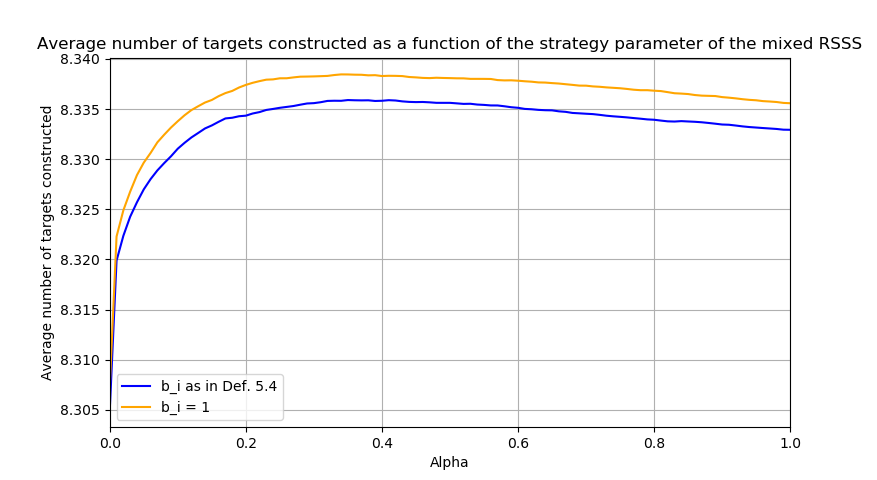
\includegraphics[scale=0.65]{images/locc_comparison.png}
    \caption{Average number of succesful target constructions depending on the value of the strategy parameter $\alpha$ for a bank of 9 uniformly sampled states (dimension 4) and 1 maximally entangled state, and 10 targets sampled with Dirichlet parameters $\left(2, \frac{1}{2}, \frac{1}{2}, \frac{1}{2}\right)$. The blue curve corresponds to the algorithm of Definition \ref{strat:uniqueness}, and the orange curve was initially a test to see if the redundancy parameter is helpful or not, and it seems not to be, which was a bit surprising. Note that on the blue curve the $\alpha = 0$ extremity is the uniqueness strategy, and $\alpha = 1$ is similar to the individual strategy, but also uses a redundancy factor $b$ and a weighted loss function $c$. For both curves, 600000 games were simulated. The entropic strategy as in Def. \ref{strat:individual} is found on the orange curve, at $\alpha = 1$, and so the curve having a maximum towards $\alpha = 0.3$ shows that we outperform the naive strategy.}
    \label{fig:strategy_comparison}
\end{figure}

\section{Discussion} \label{sec:strategies_discussion}

Eq. (\ref{eq:unique_entropy}) is computationally very demanding (which is why we didn't go over 10 states for the games, as otherwise the number of combinations is sometimes very large). Most of the time, Prop. \ref{prop:q_absorption} allows most states to vanish from the computation and the number of combinations is low enough that the computation time is manageable. However, sometimes a target such that many states fall into $Q''$ is generated, and the uniqueness entropy computation is costly.

Although the variations are not very large (less than 1\%), we were surprised that the uniqueness strategy performed worse than the entropic strategy. However, it is very interesting to see that there exists a nontrivial maximum at around $\alpha = 0.3$, where combining both the uniqueness entropy loss function and the entropic loss function performs better than a simple individual strategy. This seems to validate our lattice-based approach and the utility of $E^+$, and the mathematical theory of incomparability that we have discussed in this manuscript. Moreover, drastically different results can be reached by changing some of the state filtering choices in step \ref{step:volume}, and we believe that further research might lead to better filterings or weigthed loss functions which could further improve the performance of the different strategies. The results for another filtering (which is closer to our original vision) is shown in Appendix \ref{app:alternative_filterings}.
